%%「論文」,「レター」,「レター(C分冊)」,「技術研究報告」などのテンプレート
%% v3.4 [2023/09/12]
%% 1. 「論文」
\documentclass[paper]{ieicej}
% \documentclass[invited]{ieicej}% 招待論文
%\documentclass[survey]{ieicej}% サーベイ論文
%\documentclass[comment]{ieicej}% 解説論文
\usepackage[dvipdfmx]{graphicx,xcolor}
%%\usepackage[dvips]{graphicx}
\usepackage[fleqn]{amsmath}
%\usepackage{amsthm}
\usepackage{newtxtext}% 英数字フォントの設定を変更しないでください
\usepackage[varg]{newtxmath}% % 英数字フォントの設定を変更しないでください
%\usepackage{amssymb}
%\usepackage{bm}
\usepackage{listings,jvlisting} %日本語のコメントアウトをする場合jvlisting(もしくはjlisting)が必要
%ここからソースコードの表示に関する設定
\lstset{
  basicstyle={\ttfamily},
  identifierstyle={\small},
  commentstyle={\smallitshape},
  keywordstyle={\small\bfseries},
  ndkeywordstyle={\small},
  stringstyle={\small\ttfamily},
  frame={tb},
  breaklines=true,
  columns=[l]{fullflexible},
  numbers=left,
  xrightmargin=0zw,
  xleftmargin=3zw,
  numberstyle={\scriptsize},
  stepnumber=1,
  numbersep=1zw,
  lineskip=-0.5ex,
  % extendedchars=false, % ★ 日本語の縦書き化を防止
}
\renewcommand{\lstlistingname}{プログラム}% ソースコードのキャプションの名称

\setcounter{page}{1}

\field{A}
\jtitle{状態遷移図ベースのコード生成とログ可視化機能を備えたセンサネットワーク実機検証基盤の開発}
\etitle{}
\authorlist{%
 \authorentry{辻村篤志}{Atsushi Tsujimura}{信州大学}\MembershipNumber{}
 \authorentry{小林侑生}{Yu Kobayashi}{信州大学}\MembershipNumber{}
 \authorentry{不破泰}{Yasushi Fuwa}{信州大学}\MembershipNumber{}
 \authorentry{アサノデービッド}{David Asano}{信州大学}\MembershipNumber{}
 %\authorentry{和文著者名}{英文著者名}{所属ラベル}\MembershipNumber{}
 %\authorentry[メールアドレス]{和文著者名}{英文著者名}{所属ラベル}\MembershipNumber{}
 %\authorentry{和文著者名}{英文著者名}{所属ラベル}[現在の所属ラベル]\MembershipNumber{}
}
\affiliate[Nagano]{信州大学, 長野県}
 {Shinshu University, 4--17--1 Wakasato, Nagano-shi, 
  Nagano 380--8553 Japan}
%\affiliate[所属ラベル]{和文所属}{英文所属}
%\paffiliate\[]{}
%\paffiliate[現在の所属ラベル]{和文所属}
\jalcdoi{???????????}% ← このままにしておいてください

\begin{document}
\begin{abstract}
%和文あらまし 500字以内
センサネットワークの開発は幅広い専門知識と多大な工数を要する。先行研究では、センサネットワークの動作を表す状態遷移図からコードを生成し、汎用ハード上で動作する環境が構築されてきた。本研究ではその環境を拡張し、その上で実用的な無線通信プロトコルを実装・検証した。その過程で汎用ハード上でのプロトコルの動作が確認しづらいことを課題として認識し、デバッグ用ログ出力とそれを可視化・ステップ実行できる環境を開発しデバッグ効率の向上を図った。
\end{abstract}
\begin{keyword}
%和文キーワード 4〜5語
無線センサーネットワーク、無線通信プロトコル、状態遷移図、コード生成、ログ可視化
\end{keyword}

\begin{eabstract}
%英文アブストラクト 100 words
The development of sensor networks requires extensive expertise and significant effort. Previous research has generated code from state transition diagrams representing the behavior of sensor networks, establishing an environment that operates on general-purpose hardware. This study expands that environment and implements and verifies practical wireless communication protocols. During this process, we recognized the difficulty in confirming the operation of protocols on general-purpose hardware as a challenge and developed an environment for debugging log output and visualizing and step-executing it to improve debugging efficiency.
\end{eabstract}

\begin{ekeyword}
%英文キーワード
wireless sensor networks, wireless communication protocols, state transition diagrams, code generation, log visualization
\end{ekeyword}
\maketitle

\section{はじめに}
\subsection{背景}
近年、無線センサネットワーク(Wireless Sensor Network:WSN)は、環境モニタリングやスマートシティ、インフラ監視、農業、ヘルスケアなど、さまざまな分野での応用が期待されている。実際、WSNを含むIoTデバイスの数は2020年時点で約130億台に達し、年率20%で増加しており、2025年には300億台弱に到達すると予測されている\cite{jst2022}. また、MDPIの報告によれば、WSNノードの数は2012年の約4.5億台から2022年には約20億台へと拡大しており\cite{mdpi2021}、その研究および実用の両面での発展が顕著である。  
しかし、これらのシステムを構築するためには、複雑な通信プロトコル設計やデータ処理アルゴリズムの実装が求められ、開発者には高度な専門知識と多大な工数が必要となる。そのため、システム開発の効率化や開発者支援を目的とした研究が進められている。
\vskip\baselineskip

\subsection{従来研究}
従来研究では、無線通信プロトコルの状態遷移図から自動生成したプログラムを汎用ハード上で動作させ、CSMAおよびTDMAベースのMACプロトコルを実機で実装・検証できる環境が構築されていた(旭ら)。このシステムにより基本的な通信プロトコルの動作検証が可能となったが、デバッグ方法はシリアルコンソールへのログ出力に依存しており、通信処理が高速に進むため逐次的な状態遷移を追跡することが難しかった。その結果、異常動作の原因を把握しづらく、開発効率や教育的利用の観点では十分でない点が課題として残されていた。

\vskip\baselineskip
\subsection{目的}
本研究の目的は、従来研究で課題となっていたデバッグ効率の低さを改善し、実機でのプロトコル検証をより効果的に行える環境を実現することである。そのために、状態遷移図から生成したコードの動作をログとして出力し、それを可視化・ステップ実行できる仕組みを開発した。これにより、プロトコルの動作を逐次的に把握でき、異常動作の原因究明を容易にするとともに、教育や応用実証に適した支援環境を提供することを目指す。
\vskip\baselineskip





\section{提案システム}
\subsection{システム構成}
本研究で開発したシステムの全体構成を図\ref{fig:system-composition}に示す。本システムは、状態遷移図を入力としてC++プログラムを自動生成し、PlatformIO上でビルドを行い、汎用ハードウェア上で実行することでセンサネットワークのプロトコルの動作検証を可能とする。さらに、通信動作の状態遷移や変数値の過程をログとして記録し、ブラウザ上で状態遷移の可視化およびステップ実行を行える環境を備えている。これにより、プロトコル設計から実機検証、デバッグまでを一貫して支援することが可能となる。
\vskip\baselineskip
\begin{figure}[tb]
  \centering
  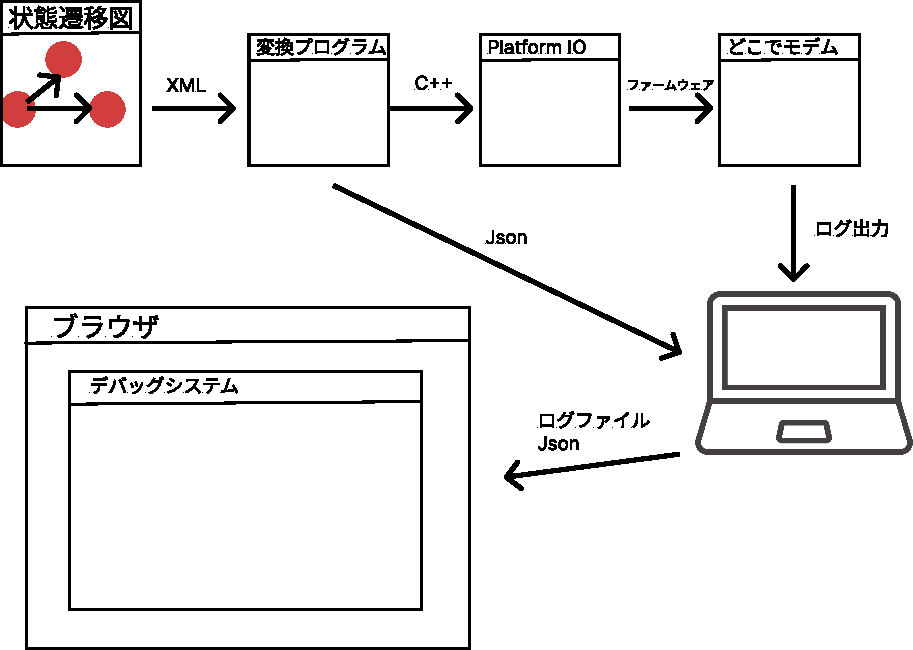
\includegraphics[width=80mm]{./images/system-composition.pdf}
  \caption{提案システムの全体構成}
  \ecaption{Block diagram of the proposed system.}
  \label{fig:system-composition}
\end{figure}


\subsection{ファームウェア生成部}
ファームウェア生成部では,無線通信プロトコルの動作をAstah Professional上の状態遷移図として設計し,XML形式で出力する。次に,変換プログラム(Python)を用いて状態遷移図のXMLをC++プログラムへ変換し,PlatformIO環境でビルドすることでファームウェアを生成する。このファームウェアは2.3節で述べる汎用ハードウェア上で実行される。

先行研究(小林ら\cite{kobayashi2023})では,状態遷移図の各要素(通信状態・遷移・初期値設定・処理内容など)をXMLファイルから抽出し,それぞれをリスト化したうえで,通信状態間の関係を解析し,C++の`switch-case`構造に変換するアルゴリズムが実装されている。本研究におけるファームウェア生成部は,この変換処理を利用しており,状態遷移図で設計されたプロトコル仕様を汎用ハードウェア上で動作するプログラムとして自動生成するものである。

図\ref{fig:state-machine}に状態遷移図の例を,プログラム\ref{converted-code}に変換後のC++コードを示す。状態遷移図で定義された「待機(LISTEN)」「受信(RECEIVE)」「送信(TRANSMIT)」の各状態と遷移関係が,`switch-case`構造によって対応づけられており,設計段階の論理構造がソースコードとして正しく反映されていることが確認できる。

\vskip\baselineskip
\begin{figure}[tb]
  \centering
  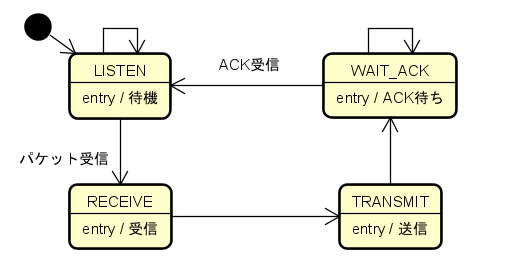
\includegraphics[width=60mm]{./images/state-machine-image.png}
  \caption{状態遷移図の例}
  \ecaption{State transition diagram.}
  \label{fig:state-machine}
\end{figure}

\begin{figure}
\begin{lstlisting}[caption={変換されたC++プログラム}, label=converted-code]
typedef enum { LISTEN, RECEIVE, TRANSMIT } NodeState;

void protocol_main() {
  switch (state) {
    case LISTEN:   updateState(RECEIVE);   break;
    case RECEIVE:  updateState(TRANSMIT);  break;
    case TRANSMIT: updateState(LISTEN);    break;
  }
}
\end{lstlisting}
\end{figure}
\vskip\baselineskip




\subsection{実行環境(ハードウェア)}
- SAMD21マイコン搭載の無線モデムであるどこでモデム(株式会社サーキットデザイン製)
- GPSモジュールによる位置情報の取得及び1PPS同期
- 複数端末での通信プロトコル動作検証
- このモデムは429MHZ帯で、汎用的(不破先生のメール参照)

次に,実行環境について述べる。本システムでは,SAMD21マイコンを搭載した無線モデム(株式会社サーキットデザイン製どこでモデム)を用い,生成したファームウェアを実行する。さらに,GPSモジュールを利用することで,位置情報の取得および1PPS信号による高精度同期を行う。これにより,複数端末間での通信プロトコル動作の検証が可能となる
\begin{figure}[tb]
  \centering
  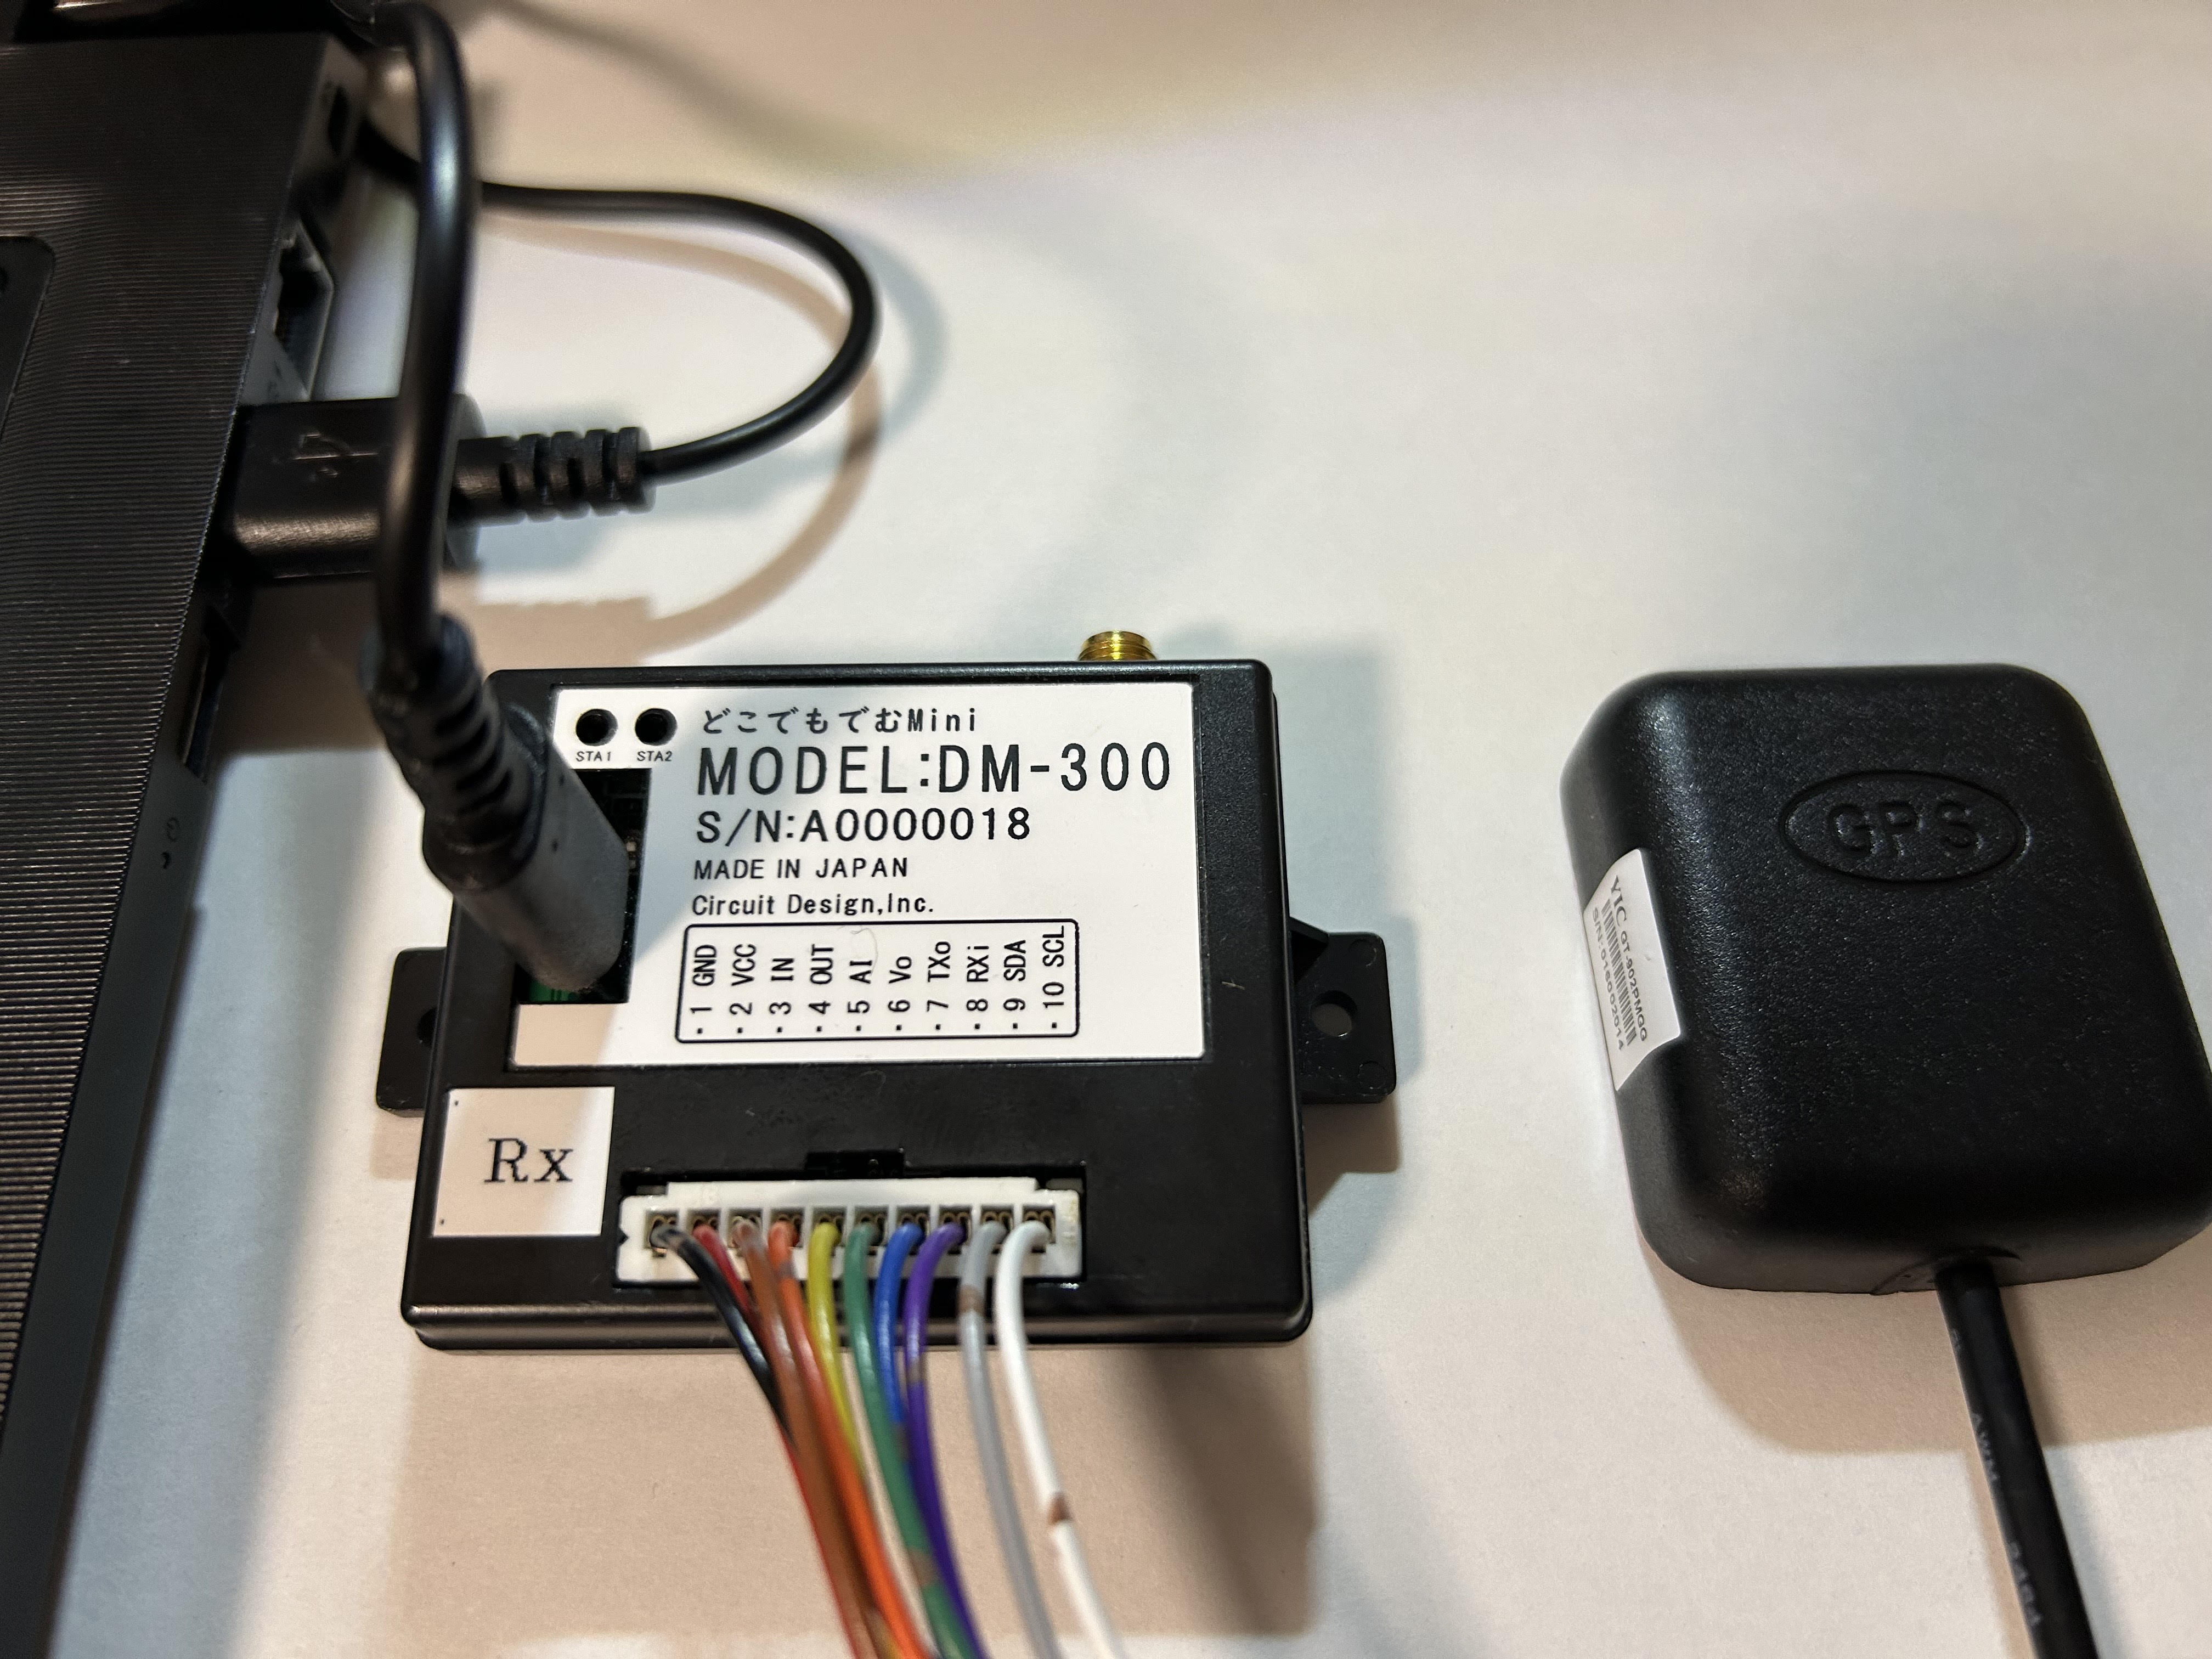
\includegraphics[width=60mm]{./images/devices.jpg}
  \caption{どこでモデム(左)とGPSモジュール(右)}
  \ecaption{Block diagram of the proposed system.}
  \label{fig:system}
\end{figure}

\subsection{デバッグシステム部}
- 通信処理時のログを逐次出力→ログファイルに書き込み(ログファイルの形式も載せるか)
- ブラウザ上でMermaid.jsにより、状態遷移図を描画(Mermaid.js用のjson?)
- ブラウザ上でログをアップロードし、ログの状態遷移を再現
- ステップ実行によるデバッグ効率の向上
- 特定の変数を追従することもできる
- リアルタイムバージョン(MQTT \& Socket)

最後に,ログ出力と可視化環境について述べる。本システムでは,通信処理時の挙動を逐次ログとして出力し,ログファイルに保存する。記録されたログをブラウザ上にアップロードすることで,Mermaid.jsを用いた状態遷移の可視化とステップ実行を可能とした。これにより,通信処理の逐次的な挙動を直感的に把握でき,デバッグ効率の大幅な向上が期待できる。また,拡張として,MQTTおよびSocket通信を用いたリアルタイム可視化の試作も行っている(状態遷移速すぎるが)。
% UIの画像
% ステップ実行の画像

\section{プロトコル実装と評価}
本システムの有効性を確認するため,状態遷移図から自動生成したコードを用いて無線通信プロトコルを実装し,複数端末間での通信を行った。その際に出力されるログをブラウザに取り込み可視化することで,プロトコルの状態遷移を逐次的に追跡できることを確認した。

従来はコンソール出力のみに依存していたため,高速に進行する通信処理の挙動を逐一把握することは困難であった。本システムではログを視覚的に再現し,ステップ実行形式で確認できるため,デバッグ効率の向上に寄与することを示した。
% デバッグ方法の比較画像
\begin{figure}[tb]
  \centering
  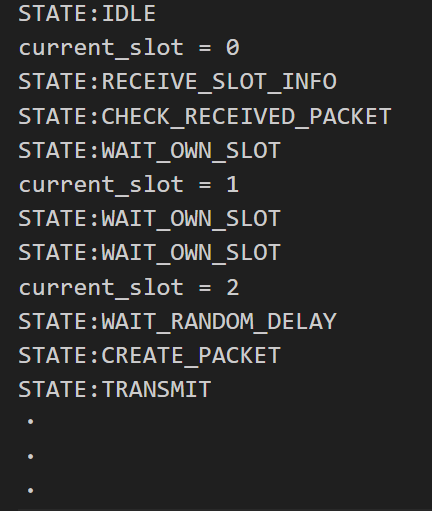
\includegraphics[width=50mm]{./images/old_debug.png}
  \caption{従来のコンソールによるデバッグ方法}
  \ecaption{Example of the old console-based debugging method.}
  \label{fig:old-debug}
\end{figure}

\section{考察}
本研究で開発したログ可視化機能により,通信処理中の状態遷移を逐次的に追跡できることを確認した。これにより,従来はコンソール出力のみに依存していたため把握が困難であったプロトコルの挙動を直感的に理解でき,デバッグ効率の向上に有効であると考えられる。

特に,従来のコンソールログによる確認方法では,高速に進行する通信処理の流れを逐一追跡することが難しく,異常動作の原因把握に時間を要していた。これに対し,本研究の可視化環境では状態遷移を図として再現できるため,通信処理の理解や他者への説明が容易になり,教育的利用や共同開発の場においても有効性が高いと考えられる。
(従来のコンソールでのデバッグと、比較した画像添付)

一方で,本研究では通信性能の定量的な評価や大規模ネットワークでの検証は行っておらず,開発環境の有効性を示すには今後さらなる検証が必要である。また,ログ可視化のリアルタイム性についても限定的であり,実時間での挙動確認に向けた拡張が今後の課


\section{まとめ、今後の展望}
本研究では,状態遷移図から生成したファームウェアを汎用ハードウェア上で実行し,無線通信プロトコルの動作を検証可能とするシステムを開発した。さらに,通信処理の挙動をログとして記録し,ブラウザ上で可視化・ステップ実行できる環境を実装することで,プロトコルの状態遷移を逐次的に追跡できることを確認した。その結果,従来のコンソール出力のみの手法と比べてデバッグ効率の向上に有効であることを示した。

今後の課題としては,定量的な評価による有効性の測定,複数端末を用いた大規模環境での検証,およびリアルタイムでのログ可視化機能の強化が挙げられる。また,登山者見守りシステムへの応用や教育現場での利用など,社会的実装を意識した展開も検討していく予定である。(ほかのセンサ導入とかも)


\vskip2\baselineskip
%\bibliographystyle{sieicej}
%\bibliography{myrefs}
\bibliographystyle{junsrt}
\begin{thebibliography}{99}
\bibitem{jst2022} 科学技術振興機構: 「SIP IoE 年次報告書 2022」, 2022.
\bibitem{mdpi2021} M. R. Hasan et al.: "Recent Advancement of Data-Driven Models in Wireless Sensor Networks," *Technologies*, vol.9, no.4, 2021.
\bibitem{asahi}
\bibitem{kobayashi2023} 小林遼, アサノデービッド, 不破泰:
“センサーネットワーク検証システムにおける遷移図を用いたMACプロトコル設計環境の開発,”
信学技報, NS2023-xx, 2023.

\bibitem{PlatformIO}
\bibitem{circuitdesign}
\bibitem{astah}
\bibitem{mermaid}
\end{thebibliography}

\appendix
\section{}

\end{document}


